\documentclass{article} % article doctype, possible font size range from 8pt to 20pt with not all being avaiable.
\title{\huge Willy The Robot Technical Design Q1-Q2 2019}
\author{Jeroen van 't Hul\\S1139163  \and Thomas Zwaanswijk\\s1089273 \and Tom van den Noort\\s1101124}
\date{\parbox{\linewidth}{\centering
	\today\endgraf\bigskip
	Supervisor \hspace*{3cm} Main Stakeholder \endgraf\medskip
	Mischa Mol \hspace*{3cm} Ilja Clabbers \endgraf\bigskip
	Windesheim Zwolle\endgraf}} 


% include packages
\usepackage{graphicx}
\usepackage{caption}
\usepackage{mathabx}
\usepackage{wrapfig}
\usepackage[margin=1.0in]{geometry} % sets page margin, 2.0in is default.
\usepackage{titlesec}
\usepackage{hyperref}
\usepackage[table,xcdraw]{xcolor}
\usepackage{float}
\usepackage[export]{adjustbox}
\usepackage{todonotes}
\usepackage{indentfirst}
\usepackage{blindtext}
\usepackage{scrextend}
\usepackage{listings}
%\usepackage{siunitx}
%\usepackage{multirow}	% used for table multirow support
%\usepackage{longtable} % Allows tables to roll over into a new page.
\usepackage[nottoc,numbib]{tocbibind} % Adds bibliography / references to TOC and numbers that section.
\usepackage{array}
\usepackage{footnote}

% ----- custom commands ----- %
% Wrapper for paragraph command. Forces newline after paragraph title
\newcommand{\myparagraph}[1]{\paragraph{#1}\mbox{}\\} % Without \mbox{} all newlines will be ignored, making the first sentence appear on the same line as a paragraph title.
% monospace codeblock
\def\code#1{\texttt{#1}}
% changing the ToC depth in the document enviroment
\newcommand{\changelocaltocdepth}[1]{%
	\addtocontents{toc}{\protect\setcounter{tocdepth}{#1}}%
	\setcounter{tocdepth}{#1}%
}

\newcolumntype{L}[1]{>{\raggedright\let\newline\\\arraybackslash\hspace{0pt}}m{#1}}
\newcolumntype{C}[1]{>{\centering\let\newline\\\arraybackslash\hspace{0pt}}m{#1}}
\newcolumntype{R}[1]{>{\raggedleft\let\newline\\\arraybackslash\hspace{0pt}}m{#1}}

% general listing styling
\lstset{
	numbers=left,
	breaklines=true,
	backgroundcolor=\color{gray},
	tabsize=4,
	basicstyle=\ttfamily,
}

\makesavenoteenv{tabular}
\makesavenoteenv{table}

\setcounter{tocdepth}{2} % only part,chapters,sections, subsections appear in ToC

\addtokomafont{labelinglabel}{\sffamily}

\DeclareCaptionFormat{cancaption}{#1#2#3\par} % Normal format actually
\DeclareCaptionLabelFormat{cancaptionlabel}{#1}
\captionsetup[figure][number]{format=cancaption,labelformat=cancaptionlabel}
\graphicspath { {images/}{../images/} }

\begin{document}
\maketitle

\begin{figure}[H]
\centering
\includegraphics[width=12 cm]{WTRLogo.png}
\end{figure}
\thispagestyle{empty}
\newpage
\setcounter{page}{1}
\tableofcontents
\newpage

% Sections
\section{Introduction}
This research is meant to create an inventory of the current state of the movements WTR\ref{trm::WTR} is capable of performing.
In addition, this document contains a list of proposed improvements in order to increase the accuracy of the autonomous driving.
By creating a list of the range of movement WTR can perform and noting any defects or issues with those, it should become easier to create a proper list of improvements.
Several sections will deal with the sensors, how they benefit the robot and their mounting as well.
\newpage

\section{Motor controller}

\subsection{Integration of closed loop}
In order to improve the driving capability of WTR, a closed loop controller has to be integrated in the motor controller. 
This means adding code to integrate two quadrature rotary encoders, adding the controller itself and combining it in a control model.
The control model is explained in the analysis of the current situation section 3.5.

The architecture of the software in the arduino Mega motor controller can be seen in figure \ref{fig::Motorconarc}.

\begin{figure}[H]
\centering
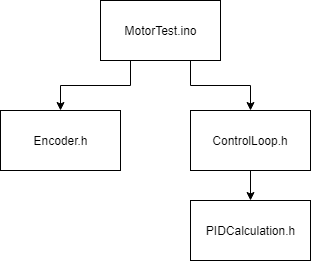
\includegraphics[width=6 cm]{MotorcontrollerArchitecture.png}
\caption{Motorcontroller architecture.}
\label{fig::Motorconarc}
\end{figure}

\subsection{Arduino Mega Code}
The main program combines sends the commands to the actual motor controller via serial bus. 
While one part of the motor controller has been made by the group, a secondary part is a pre-existing part of the original wheelchair WTR is based on.
This is considered a black box, which simply turns the brakes on and off in accordance with the commands sent from the Arduino Mega 2560.
The commands sent to the motor are refreshed at a higher frequency than the control loop is called. %why?
The flow of the main program can be found in figure \ref{fig::MPF}.

\begin{figure}[H]
\centering
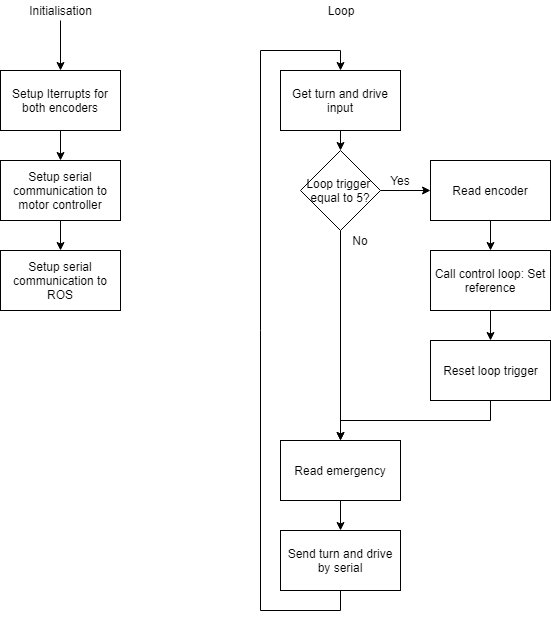
\includegraphics[width=12 cm]{MainProgramFlow.png}
\caption{Main program flow}
\label{fig::MPF}
\end{figure}


\subsection{Rotary encoders}
The rotary encoders are of the quadrature type with 256 PPR. \todo{Maybe link to a source explaining what quadrature means}
Quadrature encoders are equipped with two channels from which one is phase shifted 90 degrees compared to the second, see figure \ref{fig::QuadEnc}.
This allows a program to determine the direction in which the shaft is rotating, as well as increasing resolution.

\begin{figure}[H]
\centering
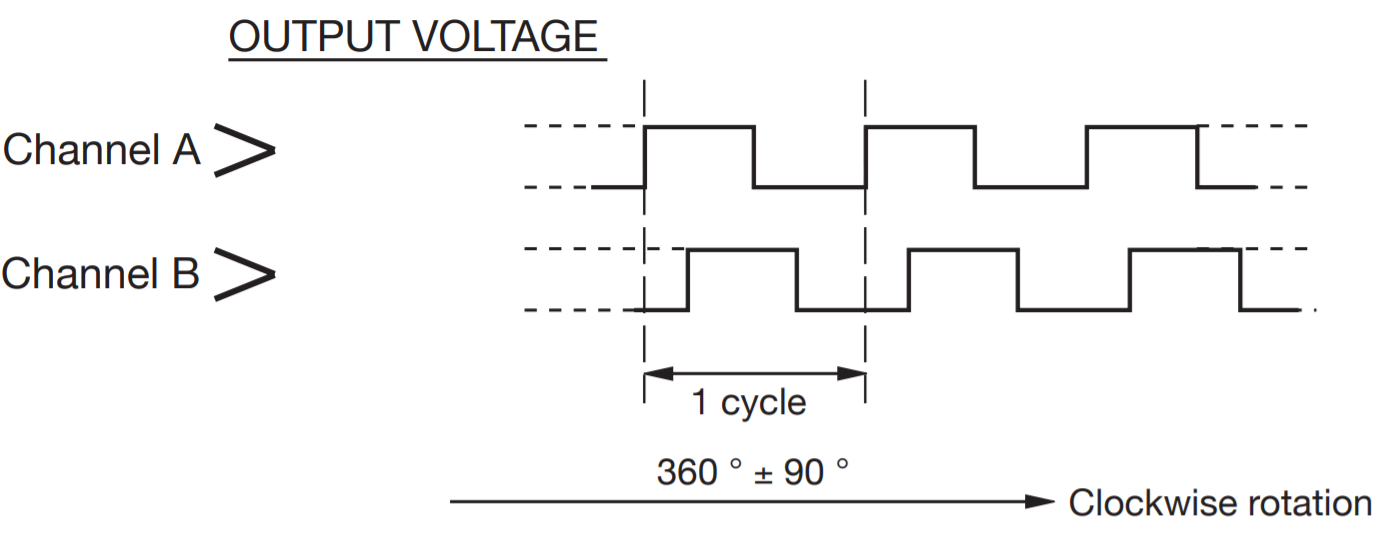
\includegraphics[width=12 cm]{QuadruatureEncoderOutput.png}
\caption{Output from quardature encoder}
\label{fig::QuadEnc}
\end{figure}


Interrupts are generated for the rising edge and for the falling edge on the pulse train per channel and therefore increase the resolution to 1024 per revolution. 
\todo{Interrupts are generated for both the rising and falling edge, which increases the resolution to 1024 pulses per revolution.}
The speed is determined using code based on the structure which can be found in the the two flowcharts below, \ref{fig::PCF} and \ref{fig::SRC}. 
The interrupt will trigger the direction determination and call a pulse change function, which stores timestamps and calculates the frequency of the pulses.
This allows the code to track the speed, and make adjustments accordingly.
This can be found in figure \ref{fig::PCF}.

When the main program wants to know the speed, it will call a speed read function which will then calculate the speed accordingly. 
This can be found in figure \ref{fig::SRC}.

\begin{figure}[H]
\centering
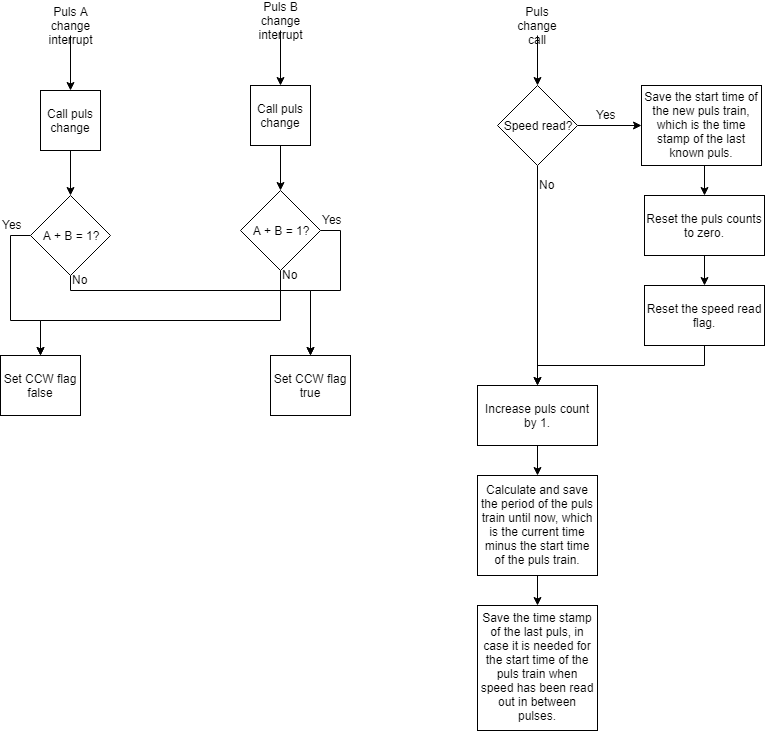
\includegraphics[width=16 cm]{Speed_determinator-Page-1.png}
\caption{Pulse change interrupt flow}
\label{fig::PCF}
\end{figure}


\begin{figure}[H]
\centering
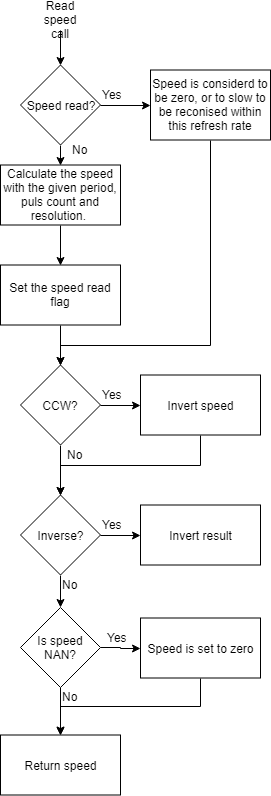
\includegraphics[width=6 cm]{Speed_determinator-Page-2.png}
\caption{Speed read call}
\label{fig::SRC}
\end{figure}

\subsection{Control loop}
The control loop calculates the speed error \ref{trm::speederror} per wheel based on feedback of the encoders and a reference \ref{trm::refturn} turn and drive input. 
This error is sent to \code{PIDCalculation()} which returns a turn and drive output. 
A detailed description of these calculations can be found in movement research. 
The flow of this class can be found in figure \ref{fig::CLF}.

\begin{figure}[H]
\centering
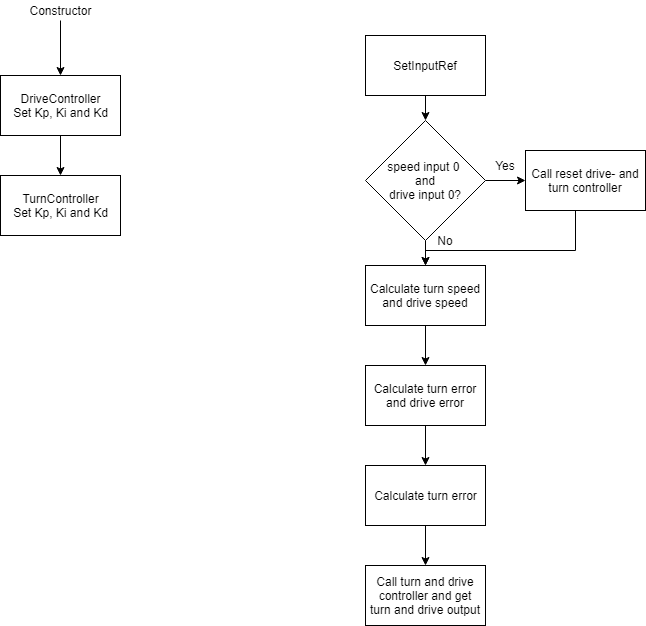
\includegraphics[width=6 cm]{ControlLoop.png}
\caption{Control loop flow}
\label{fig::CLF}
\end{figure}


\section{IMU}
The previous odometry measuring device, the MPU6250 \cite{mpu6250} was broken, which is why a new, updated version is currently being used.
Another reason a new version is used is that the MPU9250 \cite{MPU9250} also contains an AK8963, which is a 3-axis magnetometer.
This allow WTR to more accurately track orientation, since it can use the magnetometer to find its position relative to the north.
The data is collected as explained in this section \ref{sec::collect}, and then transmitted to a Raspberry Pi which deals with all the sensors.
After that has processed the data into a ROS standard message, it sends the data on to the topic, where it can then be used by planners.

\subsection{Collecting data} \label{sec::collect}
The main controller for collecting the data is an Arduino Uno, which uses I$^{2}$C for communication with the MPU9250.
The clock is set at 400000, and the address uses the \code{MPU9250\_ADDRESS\_AD0}, a macro which determines the supposed address.
In section \ref{sec::setup}, the curiosities of the address are further explained.
The Arduino takes the raw data, and uses \href{https://github.com/sparkfun/SparkFun_MPU-9250_Breakout_Arduino_Library}{this library} to process the data.
This is needed because the MPU does not output quaternions by default.
This library allows the Arduino to calculate those, and then send them on to the Pi.


\subsubsection{The Setup} \label{sec::setup}
After checking the address of the MPU9250, it will first do a self-test, where it determines the biases and stores them in its registers, through the \code{MPU9250SelfTest()} and \code{calibrateMPU9250()} functions.
The address of the MPU should be 0x71 according to the library, but since a slightly different model is used from the one the demo code is written for, the address is 0x73.
After that, it calibrates itself and stores those values as well.
Following that, it is fully initialized using the \code{initMPU9250} function.

After that, it checks what the adress of the AK8693 (the magnetometer), and if that is not 0x48, it cancels the entire system.
Thankfully, this address does match the default in the library provided.
The AK8963 is initialized, and the resolutions of the 3 different sensors are fetched using \code{getAres(), getGres(), and getMres()}.
This concludes the setup.


\subsubsection{The Loop}
The core concept of the loop is relatively simple, were it not for some of the quaternion calculations.
First it reads the data gathered by the IMU, and stores it in 3 arrays, one per sensor.
This data is then transformed, though differently per sensor.
The accelerometer data is changed to acceleration in $m/s^2$, and the gyroscopic data is calculated into degrees per second.
The magnetometer data does not get changed much, except for the compensation for the biases.

This data is then calculated into a quaternion, using the Madgwick calculation.
This is very complicated, and better to be considered as a black box.
Should you wish to learn about them anyway, consider checking out \href{http://www.ijcee.org/vol10/974-T4004.pdf}{this link}.
This does require an understanding of imaginary numbers, complex numbers, and matrix calculations.
A good source of information on those can be found \href{https://www.3dgep.com/understanding-quaternions/#The_Complex_Plane}{here.}

Of course, all the collected data in the world does not do any good if it is not transmitted, and the details on that are explained in the next section.

\subsection{Arduino to Pi protocol}
The order in which the data is sent is naturally important.
The raspberry Pi expects the data packet to start with "\$ 0x03", and then the data of the quaternion, the gyroscope, the accelerometer, the temperature and lastly the magnetometer. 

Most of the program used to interface with the MPU9250 is based on a program by sparkfun, \cite{sparkfunMPU9250}, which is in turn based on the code by KrisWiner on Github \cite{kriswiner}.
Several parts have been stripped out, since no LCD is used.
Additionally, any debug messages have been removed after confirming that the code runs consistently.

Each of the sensors returns a 16 bit piece of data, as a signed 16-bit integer.
The exception to this rule is the quaternion calculation.
For that, a float with the values ranging between -1 and +1 can be expected.
Quaternions are rather tricky to work with, but more explanation can be found \href{https://www.3dgep.com/understanding-quaternions/#The_Complex_Plane}{here.}
As a quick warning, this is rather complex math, using both imaginary numbers and matrices.
It is worthwhile to study, since they form an integral part of the message to ROS.

As serial communications are used, the data cannot be transmitted as is.
In order to combat this, the data is split into two parts, with the quaternion again being an exception.
The two 8-bit unsigned integers are then transmitted, with the 8 bits representing the MSB \ref{trm::MSB} first and the LSB \ref{trm::LSB} last.
These two integers are then spliced back into a signed 16-bit integer once the Pi has received them.


\begin{figure}[H]
    \begin{lstlisting}[language=c++,firstnumber=0]
        [ start byte ] = '$'
        [ start byte ] = 0x03
        [ quaternion value W ] = quaternion value from -1 to +1, multiplied by 100
        [ quaternion value X ]
        [ quaternion value Y ]
        [ quaternion value Z ]
        [ accelerometer X raw data high byte ]
        [ accelerometer Y raw data high byte ]
        [ accelerometer Z raw data high byte ]
        [ accelerometer X raw data low byte ]
        [ accelerometer Y raw data low byte ]
        [ accelerometer Z raw data low byte ]
        [ gyroscope X raw data high byte ]        
        [ gyroscope Y raw data high byte ]
        [ gyroscope Z raw data high byte ]
        [ gyroscope X raw data low byte ]
        [ gyroscope Y raw data low byte ]
        [ gyroscope Z raw data low byte ]
        [ magnetometer X raw data high byte ]
        [ magnetometer Y raw data high byte ]
        [ magnetometer Z raw data high byte ]
        [ magnetometer X raw data low byte ]
        [ magnetometer Y raw data low byte ]
        [ magnetometer Z raw data low byte ]
        [ message count ]
        [ '\r' ] 
        [ '\n' ] 
    \end{lstlisting} 
\caption{The order the Pi expects the data it receives to have}
\label{fig::dataformat}
\end{figure}

\subsection{Reception on the Pi}
Naturally, the data has to be sent somewhere.
In this case, the sensor Pi is responsible for handling this data.
After receiving all the data, it sends the messages to the appropriate ROS topics.

First, it creates node handles and message objects that will be used to transmit the relevant data.
The ROS communication rate is set at 200Hz, which is more than sufficient.
The covariances are set, though for the magnetometer they are as of yet unknown.
ROS uses 0.01 as a default value, 


\newpage
\section{Teb Local Planner}


\subsection{Map Drift}
One problem that has been present since the beginning of the project is something known as \textit{map drift}.
A short explanation of this problem is that the map shifts in a way that WTR is not moving.
The relative position of the map and the robot gets shifted, which throws off all planning and calculations WTR can perform.
Several methods of correction have been attempted, itemized in a list here [\ref{solist}]
\begin{itemize}
\label{solist}
\item Adding an MPU9250 - \ref{subs::mpu}
\item Tweaking configuration files of AMCL - \ref{subs::AMCL}
\item Adding plugins to RVIZ that deal with obstacle tracking and pose estimation - \ref{subs::plugins}
\item Editing the hierarchy of the Odometry and Map frames - \ref{subs::hier}
\item Reset IMU orientation every 10 seconds to lower drift between base and IMU frames - \ref{subs::reset}
\item Testing in different lighting conditions and areas - \ref{subs::light}
\item Moving the calculation of the quaternion from the Arduino the the Pi - \ref{subs::pi}
\end{itemize}
A short explanation of each of these approaches will be given in their respective subsections

\subsubsection{MPU9250}
\label{subs::mpu}
This part of the project is documented in the section [\ref{sec::IMU}].
Another IMU model, the MPU6050 was previously used.
The theory behind the implementation was that using the magnetometer, it would function to create a quaternion as well as work as a compass to give WTR a steady idea of where north is, so that it could keep better track of rotation.
This partially works, but the quaternion is not accurate enough, and there is too much EM interference for this method to be reliable.

\subsubsection{Tweaking AMCL config}
\label{subs::AMCL}
By tweaking variables such as refresh rate and the amount of rotation allowed before a rescan of obstacles, an attempt was made to reduce the drift.
The downside of this approach was that many variables are not named very well, and did not have an easily accessible explanation available.
As such, this resulted in only minor improvements.

\subsubsection{Plugins} 
\label{subs::plugins}
Due to the complex nature of RVIZ, the easiest way to add new functionality is to utilize pre-made plugins and configure those to the needs of the project.
The current set-up utilizes:
\begin{enumerate}
\item Transform (TF) tree:
    \begin{itemize}
    \item AMCL
    \item laser\_scan\_matcher
    \item laser\_filters
\end{itemize}
\item Navigation stack:
\begin{itemize}
\item move\_base
\item move\_base\_simple
\item map\_server
\item navfn
\item costmap\_2d
\item global\_planner
\item teb\_local\_planner
\end{itemize}
\end{enumerate}
Testing was done with every plugin by itself, as well as exchanging AMCL and laser\_scan\_matcher with robot\_localization\_package.
This did not result in any improvement, and the plug-ins were left as is.

\subsubsection{Hierarchy}
\label{subs::hier}
Another theory that appeared was that the problem could lie in the fact that the odometry frame in RVIZ does not move in relation to the robot, but only sporadically jumps around.
After some investigation, it became clear that this is intended behaviour, and that the odometry frame is a leftover from a now obsolete system.
As such, it seems that editing this configuration does not impact WTR, so it was left as is.

\subsubsection{Resetting Orientation}
\label{subs::reset}
Since the IMU drifts apart slowly, the theory was to reduce the drift by resetting the current position to be the \textit{zero} position, or exactly aligned with WTR's current heading.
This solution caused WTR to rotate on the map while driving straight ahead, and as such was quickly discarded.
Theoretically, this could be explored further, but it seems improbable to yield more results.

\subsubsection{Light Exposure}
\label{subs::light}
The group noticed the drift would become worse when attempting to drive WTR to the printer located on the bridge in T5.
The prevailing theory is that the amount of light and reflections from the glass are interfering with the LIDAR, since that is a light-based sensor.
Testing for this is tricky, as light from the environment is hard to get constant.
Comparisons have been made comparing an overcast day to a bright day, and during the bright day the drift was worse, but it was still present during the overcast day.

\subsubsection{Moving the Calculation}
\label{subs::pi}
The currently used calculation, the Mahoney filter, is a less intensive quaternion calculation the the Madgwick filter.
However, it is still a very complex calculation, and works best at very high speeds to eliminate drift.
The Arduino is at the very bottom tier of calculation speeds, and barely able to do this as fast as needed.
A Raspberry Pi on the other hand, has a quad-core 1GHz processor.
This speed would be more than good enough to calculate the quaternion, and even use the more accurate Madgwick version.
The problem is that the Arduino collects the data from the MPU9250, and then transmits the data to the Pi.
The Pi does not receive the data fast enough to be able to accurately calculate the quaternion, regardless of the filter used.
It results in an inaccurate quaternion which jumps around a lot due to the integration errors caused by the increased time-frame.
This was tested and then reverted back to the original set-up.

\subsection{Conclusion to the Tests}
Unfortunately, the exact cause of the drift has not been found.
Until the IMU runs well enough to be useful in the long term, turning it off in areas where the robot is far away from the odometry frame improves driving behaviour.

\newpage
\appendix % all sections after this are appendices
\section{Glossary}
\begin{itemize}
\item \label{trm::dms} Dead-man's switch - a button on a controlling unit which has to be held down in order to have the robot respond to inputs. This is generally done in order ensure a machine cannot perform any actions should the controller be dropped or receive inputs without proper supervision.
\item WTR - Willy The Robot.
\end{itemize}
% Bibliography:
\newpage
\bibliographystyle{ieeetr}
\bibliography{references}


\end{document}
